\documentclass[a4paper,12pt]{report}

\usepackage{alltt, fancyvrb, url}
\usepackage{graphicx}
\usepackage{subfigure}
\usepackage{wrapfig}
\usepackage{algorithmic}
\usepackage[utf8]{inputenc}
\usepackage{fontenc}
\usepackage{amsmath,stmaryrd,mathtools,algorithm}
\usepackage{amssymb}

% Remove option to use English naming
\usepackage[italian]{cleveref}

% Questo commentalo se vuoi scrivere in inglese.
\usepackage[italian]{babel}

\title{Meta-relazione per ``Programmazione ad Oggetti''}
 
\author{Danilo Pianini}
\date{\today}


\begin{document}
 
\maketitle

\begin{abstract}
Questo documento è una relazione di meta livello, ossia una relazione che spiega come scrivere la relazione.
%
Lo scopo di questo documento è quello di aiutare gli studenti a comprendere quali punti trattare nella loro relazione, ed in che modo farlo, evitando di perdere del tempo prezioso in prolisse discussioni di aspetti marginali tralasciando invece aspetti di maggior rilievo.
%
Per ciascuna delle sezioni del documento sarà fornita una descrizione di ciò che ci si aspetta venga prodotto dal team di sviluppo, assieme ad un elenco (per forza di cose non esaustivo) di elementi che \emph{non} dovrebbero essere inclusi.

Il modello della relazione segue il processo tradizionale di ingegneria del software fase per fase (in maniera ovviamente semplificata).
%
La struttura della relazione non è indicativa ma \textit{obbligatoria}.
%
Gli studenti dovranno produrre un documento che abbia la medesima struttura, non saranno accettati progetti la cui relazione non risponda al requisito suddetto.
%
Lo studente attento dovrebbe sforzarsi di seguire le tappe suggerite in questa relazione anche per l'effettivo sviluppo del progetto: oltre ad una considerevole semplificazione del processo di redazione di questo documento, infatti, il gruppo beneficerà di un processo di sviluppo più solido e collaudato, di tipo top-down.

La meta-relazione verrà fornita corredata di un template \LaTeX{} per coloro che volessero cimentarsi nell'uso.
%
L'uso di \LaTeX{} è vantaggioso per chi ama l'approccio ``what you mean is what you get'', ossia voglia disaccoppiare il contenuto dall'effettivo rendering del documento, accollando al motore \LaTeX{} l'onere di produrre un documento gradevole con la struttura ed il contenuto forniti.
%
L'eventuale utilizzo di \LaTeX{} non è fra i requisiti, non è parte del corso di Programmazione ad Oggetti, e non sarà ovviamente valutato. I docenti accetteranno qualunque relazione in formato standard Portable Document Format (pdf), indipendentemente dal software con cui tale documento sarà redatto.

\textbf{Nota sui diagrammi} --- Questa relazione utilizza diagrammi realizzati in notazione UML2, dove il simbolo per l'interfaccia differisce da quello di classe per la presenza di un cerchio in alto. Nella relazione che presenterete potete usare, a vostra discrezione, sia UML che UML2. Nel primo, le interfacce sono rappresentate come classi con lo stereotipo \texttt{«interface»}.
\end{abstract}

\tableofcontents
 
\chapter{Analisi}

In questo capitolo andrà fatta l'analisi dei requisiti e quella del problema, ossia verranno elencate le cose che l'applicazione dovrà fare (requisiti) e verrà descritto l'ambito in cui si colloca (analisi del problema).
%
In fase di analisi, è molto importante tenere a mente che non vi deve essere alcun riferimento al design e tantomeno alle tecnologie implementative.
%
La fase di analisi, infatti, \textit{precede} qualunque azione di design o di implementazione.

\section{Requisiti}

Nell'analisi dei requisiti si devono elencare i \emph{requisiti} dell'applicazione, ossia cosa l'applicazione dovrà fare.
%
Non ci si deve concentrare sui particolari problemi, ma esclusivamente su cosa si desidera che l'applicazione faccia.
%
È possibile descrivere separatamente i requisiti funzionali (quelli che descrivono l'effettivo comportamento dell'applicazione) da quelli non funzionali (requisiti che non riguardano direttamente aspetti comportamentali, come sicurezza, performance, eccetera).

\subsection*{Elementi positivi}
\begin{itemize}
	\item Si fornisce una descrizione in linguaggio naturale di ciò che il software dovrà fare.
	\item Gli obiettivi sono spiegati con chiarezza, per punti.
	\item Se il software è stato commissionato o è destinato ad un utente o compagnia specifici, il committente viene nominato.
	\item Se vi sono termini il cui significato non è immediatamente intuibile, essi vengono spiegati.
	\item Vengono descritti separatamente requisiti funzionali e non funzionali.
\end{itemize}

\subsection*{Elementi negativi}
\begin{itemize}
	\item Si forniscono indicazioni circa le soluzioni che si vogliono adottare
	\item Si forniscono dettagli di tipo tecnico o implementativo (parlando di classi, linguaggi di programmazione, librerie, eccetera)
\end{itemize}

\subsection*{Esempio}
Il software, commissionato dal gestore del centro di ricerca ``Aperture Laboratories Inc.''\footnote{\url{http://aperturescience.com/}}, mira alla costruzione di una intelligenza artificiale di nome GLaDOS (Genetic Lifeform and Disk Operating System).
%
Per intelligenza artificiale si intende un software in grado di assumere decisioni complesse in maniera semi autonoma sugli argomenti di sua competenza, a partire dai vincoli e dagli obiettivi datigli dall'utente.

\subsubsection{Requisiti funzionali}
\begin{itemize}
	\item La suddetta intelligenza artificiale dovrà occuparsi di coordinare le attività all'interno delle camere di test di Aperture, guidando l'utente attraverso un certo numero di sfide di difficoltà crescente. Una camera di test è un ambiente realizzato da Aperture Laboratories Inc. al fine di mettere alla prova le proprie tecnologie di manipolazione dell'ambiente. All'interno della camera di test, un soggetto qualificato è incaricato di sfruttarle per risolvere alcune sfide.
	\item Il piano preciso ed il numero delle sfide sarà variabile, e GLaDOS dovrà essere in grado di adattarsi dinamicamente e di fornire indicazioni di guida.
	\item La personalità di GLaDOS dovrà essere modificabile
	\item GLaDOS dovrà essere in grado di comunicare col reparto cucina di Aperture, per ordinare torte da donare agli utenti che completassero l'ultima camera di test con successo.
\end{itemize}

\subsubsection{Requisiti non funzionali}
\begin{itemize}
	\item GLaDOS dovrà essere estremamente efficiente nell'uso delle risorse. Le specifiche tecniche parlano della possibilità di funzionare su dispositivi alimentati da una batteria a patata.
\end{itemize}

\section{Analisi e modello del dominio}

In questa sezione si descrive il modello del dominio, descrivendo le entità in gioco ed i rapporti fra loro.
%
Si possono sollevare eventuali aspetti particolarmente impegnativi, descrivendo perché lo sono, senza inserire idee circa possibili soluzioni.

È possibile, ed è anzi raccomandato, aiutarsi con uno schema UML del dominio, che diventerà anche lo scheletro della parte ``entity'' del modello dell'applicazione (in ottica ECB - Entity Control Boundary): se l'analisi è ben fatta, dovreste ottenere una gerarchia di concetti che rappresentano le entità che compongono il problema da risolvere.
%
Un'analisi ben svolta \textbf{prima} di cimentarsi con lo sviluppo rappresenta un notevole aiuto per le fasi successive: è sufficiente descrivere a parole il dominio, quindi estrarre i sostantivi utilizzati, capire il loro ruolo all'interno del problema, le relazioni che intercorrono fra loro, e mutarli in interfacce.

\subsection*{Elementi positivi}
\begin{itemize}
	\item Viene descritto accuratamente il modello del dominio.
	\item Alcuni problemi, se non risolubili in assoluto o nel monte ore, vengono dichiarati come problemi che non saranno risolti o sarano risolti in futuro.
	\item Si modella il dominio in forma di UML.
\end{itemize}

\subsection*{Elementi negativi}
\begin{itemize}
	\item Manca una descrizione a parole del modello del dominio.
	\item Manca una descrizione UML delle entità del dominio e delle relazioni che intercorrono fra loro.
	\item Vengono elencate soluzioni ai problemi, invece della descrizione degli stessi.
	\item Vengono presentati elementi di design, o peggio aspetti implementativi.
	\item Viene mostrato uno schema UML che include elementi implementativi o non utili alla descrizione del dominio, ma volti alla soluzione (non devono vedersi, ad esempio, campi o metodi privati, o cose che non siano equivalenti ad interfacce).
\end{itemize}

\subsection*{Esempio}
GLaDOS dovrà essere in grado di accedere ad un'insieme di camere di test.
%
Tale insieme di camere prende il nome di percorso.
%
Ciascuna camera è composta di challenge successivi.
%
GLaDOS è responsabile di associare a ciascun challenge un insieme di consigli (suggestions) destinati all'utente (subject), dipendenti da possibili eventi.
%
GLaDOS dovrà poter comunicare coi locali cucina per approntare le torte.
%
Le torte potranno essere dolci, oppure semplici promesse di dolci che verranno disattese.

Gli elementi costitutivi il problema sono sintetizzati in \Cref{img:analysis}.

La difficoltà primaria sarà quella di riuscire a correlare lo stato corrente dell'utente e gli eventi in modo tale da generare i corretti suggerimenti.
%
Questo richiederà di mettere in campo appropriate strategie di intelligenza artificiale.

Data la complessità di elaborare consigli via AI senza intervento umano, la prima versione del software fornita prevederà una serie di consigli forniti dall'utente.

Il requisito non funzionale riguardante il consumo energetico richiederà studi specifici sulle performance di GLaDOS che non potranno essere effettuati all'interno del monte ore previsto: tale feature sarà oggetto di futuri lavori.

\begin{figure}
\centering{}
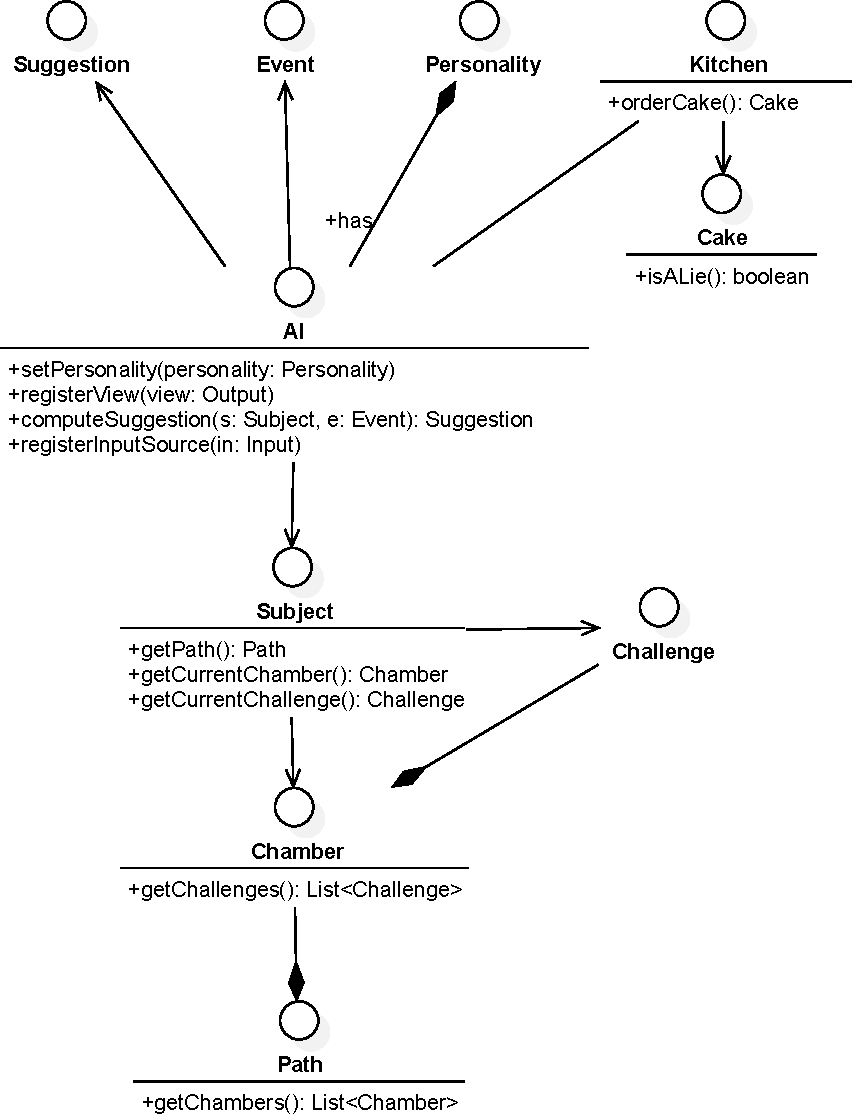
\includegraphics{img/GlaDOS__Analysis_0}
\caption{Schema UML dell'analisi del problema, con rappresentate le entità principali ed i rapporti fra loro}
\label{img:analysis}
\end{figure}

\chapter{Design}

In questo capitolo si spiegano le strategie messe in campo per realizzare la soluzione ai problemi identificati nell'analisi.

Si parte da una visione architetturale, il cui scopo è informare il lettore di quale sia il funzionamento dell'applicativo realizzato ad alto livello.
%
In particolare, è necessario descrivere accuratamente in che modo i componenti principali del sistema si coordinano fra loro.
%
A seguire, si dettagliano alcune parti del design, quelle maggiormente rilevanti al fine di chiarificare la logica con cui sono stati risolti i problemi dell'applicazione.

\section{Architettura}

Questa sezione spiega come le componenti principali del software interagiscono fra loro.
%
In particolare, qui va spiegato se e come è stato utilizzato il pattern architetturale model-view-controller (e/o entity-control-boundary).
%
Se non è stato utilizzato, va spiegata in maniera molto accurata l'architettura scelta, giustificandola in modo appropriato.

Raccomandiamo di sfruttare la definizione del dominio fatta in fase di analisi per capire quale sia l'entry point del model, e di non realizzare un'unica macro-interfaccia che, spesso, finisce con l'essere il prodromo ad una ``God class''.
%
Consigliamo anche di separare bene controller e model, facendo attenzione a non includere nel secondo strategie d'uso che appartengono al primo.
%
Infine, attenzione al design dell'interazione fra view e controller: se ben progettato, sostituire in blocco la view non dovrebbe causare alcuna modifica nel controller.

\subsection*{Elementi positivi}
\begin{itemize}
 \item Si mostrano pochi, mirati schemi UML dai quali si deduce con chiarezza quali sono le parti principali del software e come interagiscono fra loro.
 \item Si mette in evidenza se e come il pattern architetturale model-view-controller è stato applicato, anche con l'uso di un UML che mostri le interfacce principali ed i rapporti fra loro.
 \item Si discute se sia semplice o meno, con l'architettura scelta, sostituire in blocco la view senza toccare minimamente il controller. Va da sé che, se cambiare la UI si trasforma in un bagno di sangue che impatta controller o modello, il design architetturale non è stato fatto in modo adeguato.
\end{itemize}

\subsection*{Elementi negativi}
\begin{itemize}
 \item L'architettura è fatta in modo che sia impossibile riusare il modello per un software diverso che affronta lo stesso problema.
 \item L'architettura è tale che l'aggiunta di una funzionalità sul controller impatta pesantemente su view e/o modello.
 \item L'architettura è tale che la sostituzione in blocco della view impatta sul controller o, peggio ancora, sul modello.
 \item Si presentano UML caotici, difficili da leggere.
 \item Si presentano UML in cui sono mostrati elementi di dettaglio non appartenenti all'architettura, ad esempio includenti campi o con metodi che non interessano la parte di interazione fra le componenti principali del software.
 \item Si presentano schemi UML con classi (nel senso UML del termine) che ``galleggiano'' nello schema, non connesse, ossia senza relazioni con il resto degli elementi inseriti.
 \item Si presentano elementi di design di dettaglio, ad esempio tutte le classi e interfacce del modello o della view.
 \item Si discutono aspetti implementativi, ad esempio eventuali librerie usate oppure dettagli di codice.
\end{itemize}

\subsection*{Esempio}
L'architettura di GLaDOS segue il pattern architetturale ECB.
GLaDOS implementa l'interfaccia AI, ed è l'effettivo controller del sistema.
Essendo una intelligenza artificiale, è una classe attiva.
GLaDOS accetta la registrazione di Input ed Output.
Gli Input rappresentano delle nuove informazioni che vengono fornite all'IA, ad esempio delle modifiche nel valore di un sensore, oppure un comando da parte dell'operatore.
Questi input infatti forniscono eventi.
Ottenere un evento è un'operazione bloccante: chi la esegue resta in attesa di un effettivo evento.
Ogni volta che c'è un cambio alla situazione del soggetto, GLaDOS notifica i suoi Output, informandoli su quale sia la situazione corrente.

Con questa architettura, possono essere aggiunti un numero arbitrario di input ed output all'intelligenza artificiale.

In \Cref{img:goodarch} è esemplificato il diagramma UML architetturale.

\begin{figure}
\centering{}
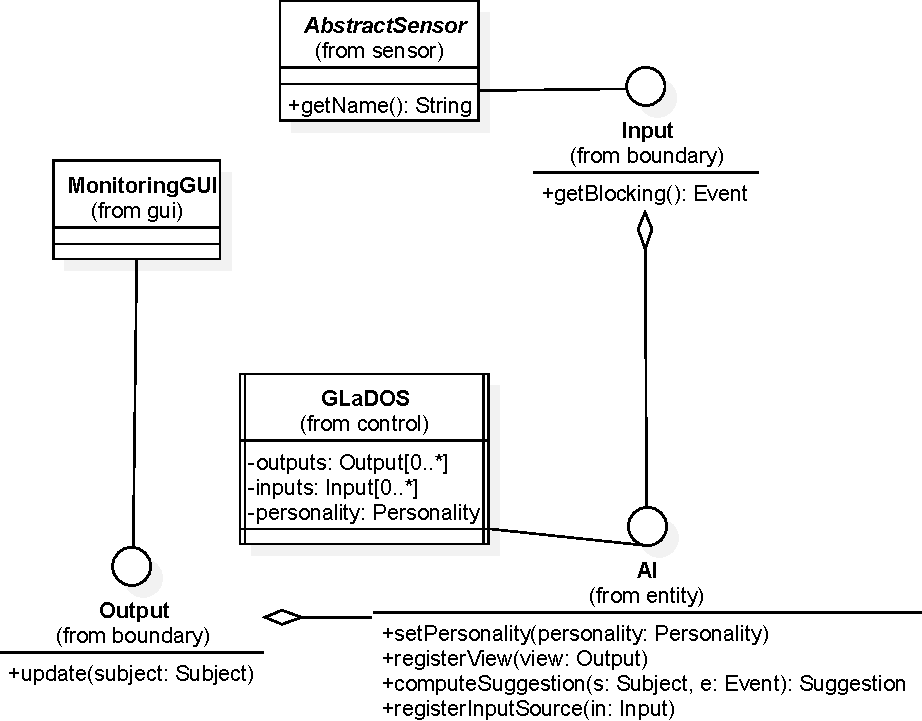
\includegraphics[width=\textwidth]{img/GlaDOS__Architecture_1}
\caption{Schema UML architetturale di GLaDOS}
\label{img:goodarch}
\end{figure}


\section{Design dettagliato}

In questa sezione si possono approfondire alcuni elementi del design con maggior dettaglio.
%
Mentre ci attendiamo principalmente (o solo) interfacce negli schemi UML delle sezioni precedenti, in questa sezione è necessario scendere in maggior dettaglio presentando la struttura di alcune sottoparti rilevanti dell'applicazione.
%
È molto importante che, descrivendo un problema, quando possibile si mostri che non si è re-inventata la ruota ma si è applicato un design pattern noto.
%
È assolutamente inutile, ed è anzi controproducente, descrivere classe-per-classe (o peggio ancora metodo-per-metodo) com'è fatto il vostro software: è un livello di dettaglio proprio della documentazione dell'API (deducibile dalla Javadoc).

\textbf{È necessario che ciascun membro del gruppo abbia una propria sezione di design dettagliato, di cui sarà responsabile}.
%
Ciascun autore dovrà spiegare in modo corretto e giustamente approfondito (non troppo in dettaglio, non superficialmente) il proprio contributo.
%
È importante focalizzarsi sulle scelte che hanno un impatto positivo sul riuso, sull'estensibilità, e sulla chiarezza dell'applicazione.
%
Usare correttamente i design pattern in questa sezione è molto importante: se vengono utilizzati, si ha la garanzia che quanto fatto sia conforme allo stato dell'arte.

Esattamente come nessun ingegnere meccanico presenta un solo foglio con l'intero progetto di una vettura di Formula 1, ma molteplici fogli di progetto che mostrano a livelli di dettaglio differenti le varie parti della vettura e le modalità di connessione fra le parti, così ci aspettiamo che voi, futuri ingegneri informatici, ci presentiate prima una visione globale del progetto, e via via siate in grado di dettagliare le singole parti, scartando i componenti che non interessano quella in esame.
%
Per continuare il parallelo con la vettura di Formula 1, se nei fogli di progetto che mostrano il design delle sospensioni anteriori appaiono pezzi che appartengono al volante o al turbo, vuol dire che c'è qualche grosso problema di design.

\subsection*{Elementi positivi}

\begin{itemize}
	\item Ogni membro del gruppo discute le proprie decisioni di progettazione, ed in particolare le azioni volte ad anticipare possibili cambiamenti futuri (ad esempio l'aggiunta di una nuova funzionalità, o il miglioramento di una esistente).
	\item Si identificano ed utilizzano numerosi design pattern.
	\item Ogni membro del gruppo identifica i pattern utilizzati nella sua sottoparte.
	\item Si mostrano gli aspetti di design più rilevanti dell'applicazione, mettendo in luce la maniera in cui si è costruita la soluzione ai problemi descritti nell'analisi.
	\item Si tralasciano aspetti strettamente implementativi e quelli non rilevanti, non mostrandoli negli schemi UML (ad esempio, campi privati) e non descrivendoli.
	\item Si mostrano le principali interazioni fra le varie componenti che collaborano alla soluzione di un determinato problema.
	\item Ciascun design pattern identificato presenta una piccola descrizione del problema calato nell'applicazione, uno schema UML che ne mostri la concretizzazione nelle classi del progetto, ed una breve descrizione della motivazione per cui tale pattern è stato scelto.
	\item La divisione in package rispecchia l'architettura e consente di navigare facilmente il sorgente, dando brevi giustificazione alle scelte fatte.
\end{itemize}

\subsection*{Elementi negativi}
\begin{itemize}
	\item Il design del modello risulta scorrelato dal problema descritto in analisi.
	\item Si tratta in modo prolisso, classe per classe, il software realizzato.
	\item Non si presentano schemi UML esemplificativi.
	\item Non si individuano design pattern, o si individuano in modo errato (si spaccia per design pattern qualcosa che non lo è).
	\item Si producono schemi UML caotici e difficili da leggere, che comprendono inutili elementi di dettaglio.
	\item Si presentano schemi UML con classi (nel senso UML del termine) che ``galleggiano'' nello schema, non connesse, ossia senza relazioni con il resto degli elementi inseriti.
	\item Si tratta in modo inutilmente prolisso la divisione in package, elencando ad esempio le classi una per una.
	\item La divisione in package non rispecchia l'architettura, o è caotica.
\end{itemize}

% \subsection*{Esempio di buona suddivisione in package}
% L'applicazione è stata divisa in tre sottoparti logiche, come descritto nell'architettura: Model, Controller e Boundary. Maggiori dettagli sulle scelte fatte:
% \begin{itemize}
%  \item Radice: non avendo alcun dominio, abbiamo deciso di utilizzare il prefisso dell'Università, cui abbiamo aggiunto un nostro identificativo: \texttt{it.unibo.studentsgroup}. Inoltre, abbiamo aggiunto un suffisso che indentifica questo progetto, per cui tutti i package saranno prefissi da: \texttt{it.unibo.studentsgroup.thisapp}.
%  \item Abbiamo diviso l'applicazione in tre sottoparti logiche in architettura, la divisione in package le rispecchia: \texttt{.model}, \texttt{.control}, \texttt{.boundary}. 
%  \item Essendo la parte di gestione dell'I/O composta di molti sorgenti, abbiamo suddiviso \texttt{.boundary} in sottopackage: \texttt{.boundary.network} e \texttt{.boundary.local}.
%  \item All'interno del model il concetto di \texttt{InterfacciaMoltoUsata} è stato implementato da numerose classi diverse. Di conseguenza, abbiamo adottato un subpackage \texttt{.model.imoltousata} dove abbiamo organizzato tutte le implementazioni, rendendo più navigable il package \texttt{it.unibo.studentsgroup.thisapp.model}.
% \end{itemize}


\subsection*{Esempi di UML ben realizzati}

In questa sezione ci si concentrerà sugli aspetti di personalità e sul funzionamento del reporting di GLaDOS.

Il sistema per la gestione della personalità utilizza il pattern Strategy, come da \Cref{img:strategy}: le implementazioni di Personality possono essere modificate, e la modifica impatta direttamente sul comportamento di GLaDOS.

\begin{figure}
\centering{}
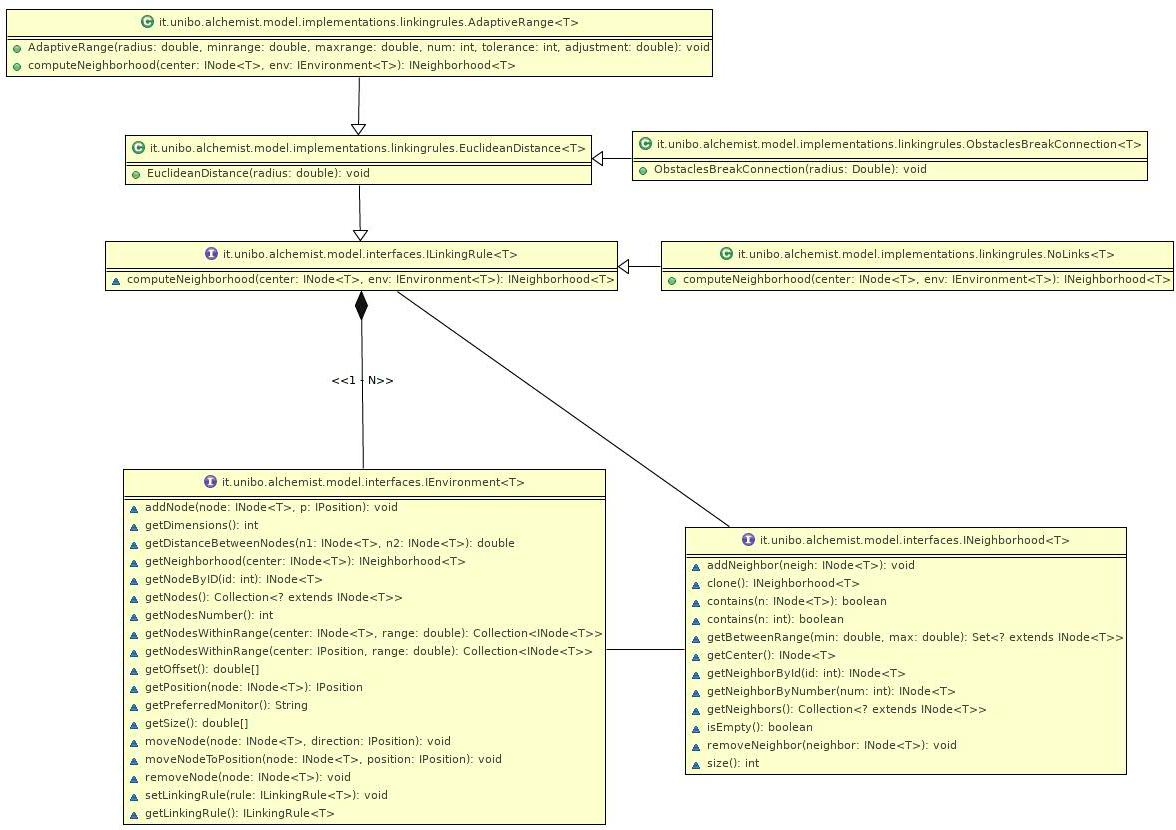
\includegraphics[width=\textwidth]{img/strategy}
\caption{Rappresentazione UML del pattern Strategy per la personalità di GLaDOS}
\label{img:strategy}
\end{figure}

Sono state attualmente implementate due personalità, una buona ed una cattiva.
Quella buona restituisce sempre una torta valida, mentre quella cattiva restituisce sempre una torta.
Dato che le due personalità differiscono solo per il comportamento da effettuarsi in caso di percorso completato con successo, è stato utilizzato il pattern template method per massimizzare il riuso, come da \Cref{img:template}.
Il metodo template è onSuccess(), che chiama un metodo astratto e protetto makeCake().

\begin{figure}
\centering{}
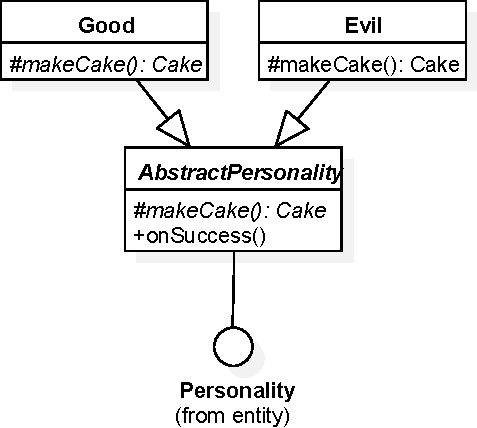
\includegraphics[width=\textwidth]{img/template}
\caption{Rappresentazione UML dell'applicazione del pattern Template Method alla gerarchia delle Personalità}
\label{img:template}
\end{figure}

Per quanto riguarda il reporting, è stato utilizzato il pattern Observer per consentire la comunicazione uno-a-molti fra GLaDOS ed i sistemi di output.
Il suo utilizzo è esemplificato in \Cref{img:observer}

\begin{figure}
\centering{}
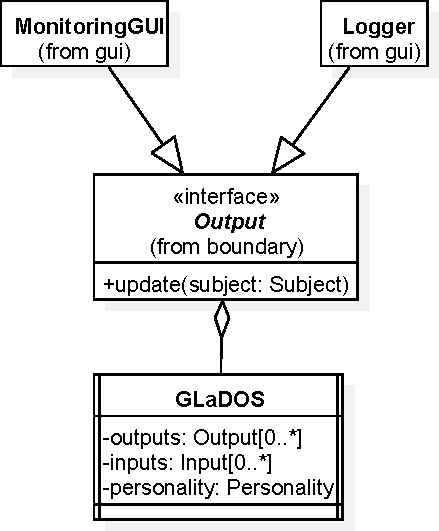
\includegraphics[width=\textwidth]{img/observer}
\caption{Il pattern Observer è usato per consentire a GLaDOS di informare tutti i sistemi di output in ascolto}
\label{img:observer}
\end{figure}

\subsection*{Esempio di pessimo diagramma UML}

In \Cref{img:badarch} è mostrato il modo \textbf{sbagliato} di fare le cose.
%
Questo schema è fatto male perché:
\begin{itemize}
	\item È caotico.
	\item È difficile da leggere e capire.
	\item Vi sono troppe classi, e non si capisce bene quali siano i rapporti che intercorrono fra loro.
	\item Si mostrano elementi implementativi irrilevanti, come i campi e i metodi privati nella classe \texttt{AbstractEnvironment}.
	\item Se l'intenzione era quella di costruire un diagramma architetturale, allora lo schema è ancora più sbagliato, perché mostra pezzi di implementazione.
	\item Una delle classi, in alto al centro, galleggia nello schema, non connessa a nessuna altra classe, e di fatto costituisce da sola un secondo schema UML scorrelato al resto
	\item Le interfacce presentano tutti i metodi e non una selezione che aiuti il lettore a capire quale parte del sistema si vuol mostrare.
\end{itemize}


\begin{figure}
\centering{}
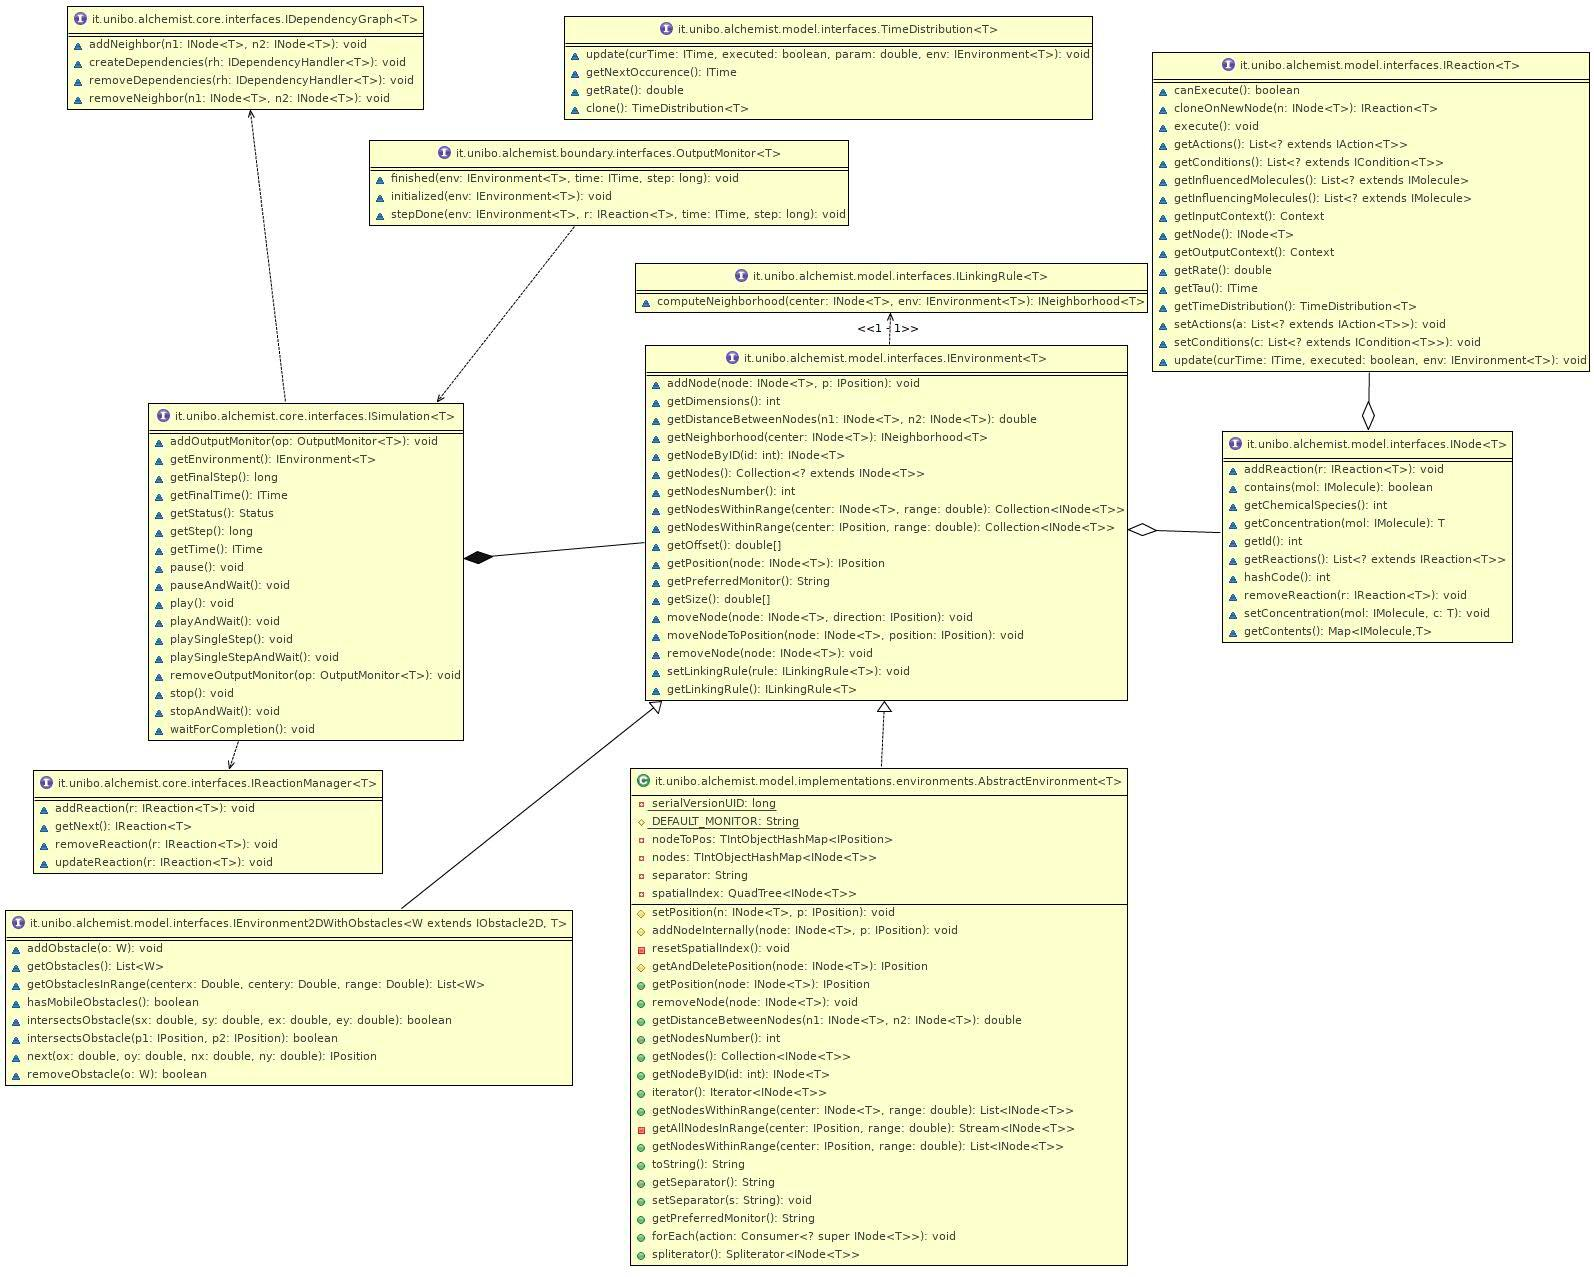
\includegraphics[width=\textwidth]{img/badarch}
\caption{Schema UML mal fatto e con una pessima descrizione, che non aiuta a capire. Don't try this at home.}
\label{img:badarch}
\end{figure}


\chapter{Sviluppo}
\section{Testing automatizzato}

Il testing automatizzato è un requisito di qualunque progetto software che si rispetti, e consente di verificare che non vi siano regressioni nelle funzionalità a fronte di aggiornamenti.
%
Per quanto riguarda questo progetto è considerato sufficiente un test minimale, a patto che sia completamente automatico.
%
Test che richiedono l'intervento da parte dell'utente sono considerati \textit{negativamente} nel computo del punteggio finale.

\subsection*{Elementi positivi}

\begin{itemize}
 \item Si descrivono molto brevemente i componenti che si è deciso di sottoporre a test automatizzato.
 \item Si utilizzano suite specifiche (e.g. JUnit) per il testing automatico.
 \item Se sono stati eseguiti test manuali di rilievo, si elencano descrivendo brevemente la ragione per cui non sono stati automatizzati. Ad esempio, se tutto il team sviluppa e testa su uno stesso sistema operativo e si sono svolti test manuali per verificare, ad esempio, il corretto funzionamento dell'interfaccia grafica o di librerie native su altri sistemi operativi, può avere senso menzionare la cosa.
\end{itemize}

\subsection*{Elementi negativi}
\begin{itemize}
 \item Non si realizza alcun test automatico.
 \item La non presenza di testing viene aggravata dall'adduzione di motivazioni non valide.
 \item Si descrive un testing di tipo manuale in maniera prolissa.
 \item Si descrivono test effettuati manualmente che sarebbero potuti essere automatizzati, ad esempio scrivendo che si è usata l'applicazione manualmente.
\end{itemize}

\section{Metodologia di lavoro}

Ci aspettiamo, leggendo questa sezione, di trovare conferma alla divisione operata nella sezione del design di dettaglio, e di capire come è stato svolto il lavoro di integrazione.

\subsection*{Elementi positivi}

\begin{itemize}
	\item Si identifica con precisione il ruolo di ciascuno all'interno del gruppo, ossia su quale parte del progetto ciascuno dei componenti si è concentrato maggiormente.
	\item La divisione dei compiti è equa, ossia non vi sono membri del gruppo che hanno svolto molto più lavoro di altri
	\item La divisione dei compiti è coerente con quanto descritto nelle parti precedenti della relazione
	\item La divisione dei compiti è realistica, ossia le dipendenze fra le parti sviluppate sono minime
	\item Si identifica quale parte del software è stato sviluppato da tutti i componenti insieme.
	\item Si spiega in che modo si sono integrate le parti di codice sviluppate separatamente, evidenziando eventuali problemi. Ad esempio, una strategia è convenire sulle interfacce da usare (ossia, occuparsi insieme di stabilire l'architettura) e quindi procedere indipendentemente allo sviluppo di parti differenti. Una possibile problematica potrebbe essere una dimenticanza in fase di design architetturale che ha costretto ad un cambio e a modifiche in fase di integrazione. Una situazione simile è la norma nell'ingegneria di un sistema software non banale, ed il processo di progettazione top-down con raffinamento successivo è il così detto processo ``a spirale''.
	\item Si descrive in che modo è stato impiegato il DVCS.
\end{itemize}

\subsection*{Elementi negativi}
\begin{itemize}
	\item Non si chiarisce chi ha fatto cosa.
	\item C'è discrepanza fra questa sezione e le sezioni che descrivono il design dettagliato.
	\item Tutto il progetto è stato svolto lavorando insieme invece che assegnando una parte a ciascuno.
	\item Non viene descritta la metodologia di integrazione delle parti sviluppate indipendentemente.
	\item Uso superficiale del DVCS.
\end{itemize}

\section{Note di sviluppo}

Questa sezione, come quella riguardante il design dettagliato va svolta \textbf{singolarmente da ogni membro del gruppo}.

Ciascuno dovrà mettere in evidenza eventuali particolarità del suo metodo di sviluppo, ed in particolare:
\begin{itemize}
	\item Elencare le feature avanzate del linguaggio Java che sono state utilizzate. Le feature di interesse possono essere, ad esempio:
	\begin{itemize}
		\item Uso avanzato dei generici (ad esempio costruzione di nuovi tipi generici, e uso di generici bounded)
		\item Uso delle lambda expressions
		\item Uso degli stream, degli optional o di altri costrutti monadici
		\item Uso della reflection
		\item Uso di parti di libreria non spiegate a lezione (networking, JavaScript via Nashorn, eccetera...)
	\end{itemize}
	Si faccia molta attenzione a non scrivere banalità, elencando qui features di tipo ``core'', come le eccezioni, o le inner class.
	\item Descrivere eventuali approfondimenti fatti rispetto a quanto trattato nel corso (ad esempio l'utilizzo di un logger, o l'accesso alla rete, o l'uso di librerie grafiche particolari)
	\item Descrivere le librerie utilizzate nella propria parte di progetto. Si ricorda che l'utilizzo di librerie è valutato \emph{positivamente}.
	\item Sviluppo di algoritmi particolarmente interessanti \emph{non forniti da alcuna libreria}
\end{itemize}

In questa sezione è anche bene evidenziare eventuali pezzi di codice scopiazzati da Internet o da altri progetti (pratica che tolleriamo ma che non raccomandiamo).

\subsection*{Elementi positivi}

\begin{itemize}
	\item Si elencano gli aspetti avanzati di linguaggio che sono stati impiegati
	\item Si elencano le librerie che sono state utilizzate
	\item Si descrivono aspetti particolarmente complicati o rilevanti relativi all'implementazione, ad esempio, in un'applicazione performance critical, un uso particolarmente avanzato di meccanismi di caching, oppure l'implementazione di uno specifico algorigmo.
	\item Se si è utilizzato un particolare algoritmo, se ne cita la fonte originale. Ad esempio, se si è usato Mersenne Twister per la generazione dei numeri random, si cita \cite{mersenne}.
	\item Si identificano parti di codice prese da altri progetti, dal web, o comunque scritte in forma originale da altre persone. In tal senso, si ricorda che agli ingegneri non è richiesto di re-inventare la ruota continuamente: se ci cita debitamente la sorgente è tollerato fare uso di di snippet di codice per risolvere velocemente problemi non banali. Nel caso in cui si usino snippet di codice di qualità discutibile, oltre a menzionarne l'autore originale si invitano gli studenti ad adeguare tali parti di codice agli standard e allo stile del progetto.
\end{itemize}

\subsection*{Elementi negativi}
\begin{itemize}
 \item Si elencano feature core del linguaggio invece di quelle segnalate.
 \item Si descrivono aspetti di scarsa rilevanza, o si scende in dettagli inutili.
 \item Sono presenti parti di codice sviluppate originalmente da altri che non vengono debitamente segnalate. In tal senso, si ricorda agli studenti che i docenti hanno accesso a tutti i progetti degli anni passati, a Stack Overflow, ai principali blog di sviluppatori ed esperti Java e ai blog dedicati allo sviluppo di soluzioni e applicazioni (inclusi blog dedicati ad Android e allo sviluppo di videogame). Conseguentemente, è \emph{molto} conveniente \emph{citare} una fonte ed usarla invece di tentare di spacciare per proprio il lavoro di altri.
\end{itemize}

\chapter{Commenti finali}

In quest'ultimo capitolo si tirano le somme del lavoro svolto e si delineano eventuali sviluppi futuri.

\section{Autovalutazione e lavori futuri}

\subsection*{Cosa scrivere}

\textbf{È richiesta una sezione per ciascun membro del gruppo}.
%
Ciascuno dovrà autovalutare il proprio lavoro, elencando i punti di forza e di debolezza in quanto prodotto.
Si dovrà anche cercare di descrivere \emph{in modo quanto più obiettivo} il proprio ruolo all'interno del gruppo.
Si ricorda, a tal proposito, che ciascuno studente è responsabile solo della propria sezione: non è un problema se ci sono opinioni contrastanti, a patto che rispecchino effettivamente l'opinione di chi le scrive.
Nel caso in cui si pensasse di portare avanti il progetto, ad esempio perché effettivamente impiegato, o perché sufficientemente ben riuscito da poter esser usato come dimostrazione di esser capaci progettisti, si descriva brevemente verso che direzione portarlo.

\section{Difficoltà incontrate e commenti per i docenti}

Questa sezione, opzionale, può essere utilizzata per segnalare ai docenti eventuali problemi o difficoltà incontrate nel corso o nello svolgimento del progetto.
%
È possibile che alcuni dei commenti forniti vengano utilizzati per migliorare il corso in futuro: sebbene non andrà a vostro beneficio, potreste fare un favore ai vostri futuri colleghi.
%
Ovviamente il contenuto della sezione non impatterà il voto finale.

\appendix
\chapter{Guida utente}

Capitolo in cui si spiega come utilizzare il software. Nel caso in cui il suo uso sia del tutto banale, tale capitolo può essere omesso.

\subsection*{Elementi positivi}

\begin{itemize}
 \item Si istruisce in modo semplice l'utente sull'uso dell'applicazione, eventualmente facendo uso di schermate e descrizioni.
\end{itemize}

\subsection*{Elementi negativi}
\begin{itemize}
 \item Si descrivono in modo eccessivamente minuzioso tutte le caratteristiche, anche minori, del software in oggetto.
 \item Manca una descrizione che consenta ad un utente qualunque di utilizzare almeno le funzionalità primarie dell'applicativo.
\end{itemize}

\bibliographystyle{abbrv}
\bibliography{template}

\end{document}